% vim: fo=aw2tq tw=100 spell
\documentclass[10pt]{article}
\setlength{\parskip}{0.5\baselineskip}

% Necessary packages
%\usepackage{pslatex}
\usepackage[T1]{fontenc}
\usepackage{lmodern}
\renewcommand*\ttdefault{txtt}
%\usepackage[scaled]{beramono}
%\usepackage{textcomp}
%\usepackage{pxfonts}
%\usepackage{bookman}

\usepackage{listings}
\usepackage{shortvrb}
\usepackage[pdftex]{color,graphicx}
\usepackage[pdftex]{hyperref}

% Use "foo" for short verbatim
\MakeShortVerb{\"}

% Coloured links, not frames
\hypersetup{colorlinks=true}

% Define a listings language for h180
\lstdefinelanguage{h180}{
    keywordsprefix=.,
    keywords={add,adc,and,cp,cpl,dec,inc,mlt,neg,or,sub,sbc,tst,xor,rl,rla,rlc,rlca,rr,rra,rrc,
rrca,rld,rrd,sla,sra,srl,set,res,bit,ld,cpd,cpdr,cpi,cpir,ldd,lddr,ldi,ldir,push,pop,ex,exx,call,
djnz,jp,jr,ret,reti,retn,rst,in,in0,ind,indr,ini,inir,out,out0,otdm,otdmr,otdr,outi,otir,tstio,otim,
otimr,outd,daa,ccf,scf,di,ei,halt,im,nop,slp},
    sensitive=false,
    comment=[l]{\#},
}
% Define the h180 environment
\lstnewenvironment{h180}{\lstset{language=h180}}{}
% Define the global listing style
\lstset{lineskip=-1pt, basicstyle=\small\ttfamily, frame=lines, framerule=0.2pt}


% Document info
\title{Microcomputer Communications Project (MCP)}
\author{Examination number: Y2265520}
% TODO: Lab partner's examination number!!!

\begin{document}

% Title page
\maketitle
%\vfill
\begin{center}
1234 words
\end{center}
\pagebreak
% Table of Contents
\tableofcontents

% vim: fo=aw2tq tw=100 spell
\section{Introduction}

The aim of the project is the development and implementation of an embedded system capable of 
synthesising one or more musical instruments, and playing these instruments in a real-time manner 
based on a serial network data stream.

The base hardware supplied for this task is a Single-Board Computer (SBC) based on the Hitachi 64180 
CPU --- a Z180 clone, which in turn is an extended Z80, with a few extra instructions and most of 
the useful peripherals built in (serial I/O controller, DMA controller, programmable reload timers).  
This CPU is clocked faster than the Z80, at 6.144MHz, and has a physical address space of 512kB 
courtesy of a programmable Memory Management Unit (MMU), but shares the Z80's 64kB logical address 
space since the instruction set only allows 16-bit memory addresses.  Some instructions have also 
been implemented more efficiently, requiring fewer clock cycles to complete.

In addition to the 64180 chip, many other useful peripherals are part of the SBC, including an 
I$^{2}$C controller, Real-Time Clock (RTC), 24-bit parallel digital I/O, 4-bit hexadecimal keypad 
and $16\times2$ character LCD text display.  The board is fitted with 96kB of RAM, and a ROM 
containing a very basic operating system that, among other things, supports loading software over a 
serial connection and starting execution at a specified memory location.

% TODO: More info on the output
Output is to be via a supplied $8\Omega$ impedance speaker.  Any other hardware required for the 
output is to be designed and built jointly with a partner, since repeated changing of hardware on a 
shared system for testing individual solutions is impractical, and the design of the hardware will 
heavily influence the way in which the software is written.

% vim: fo=aw2tq tw=100 spell
\section{Functional Overview}

\begin{figure}[htbp]
\centering
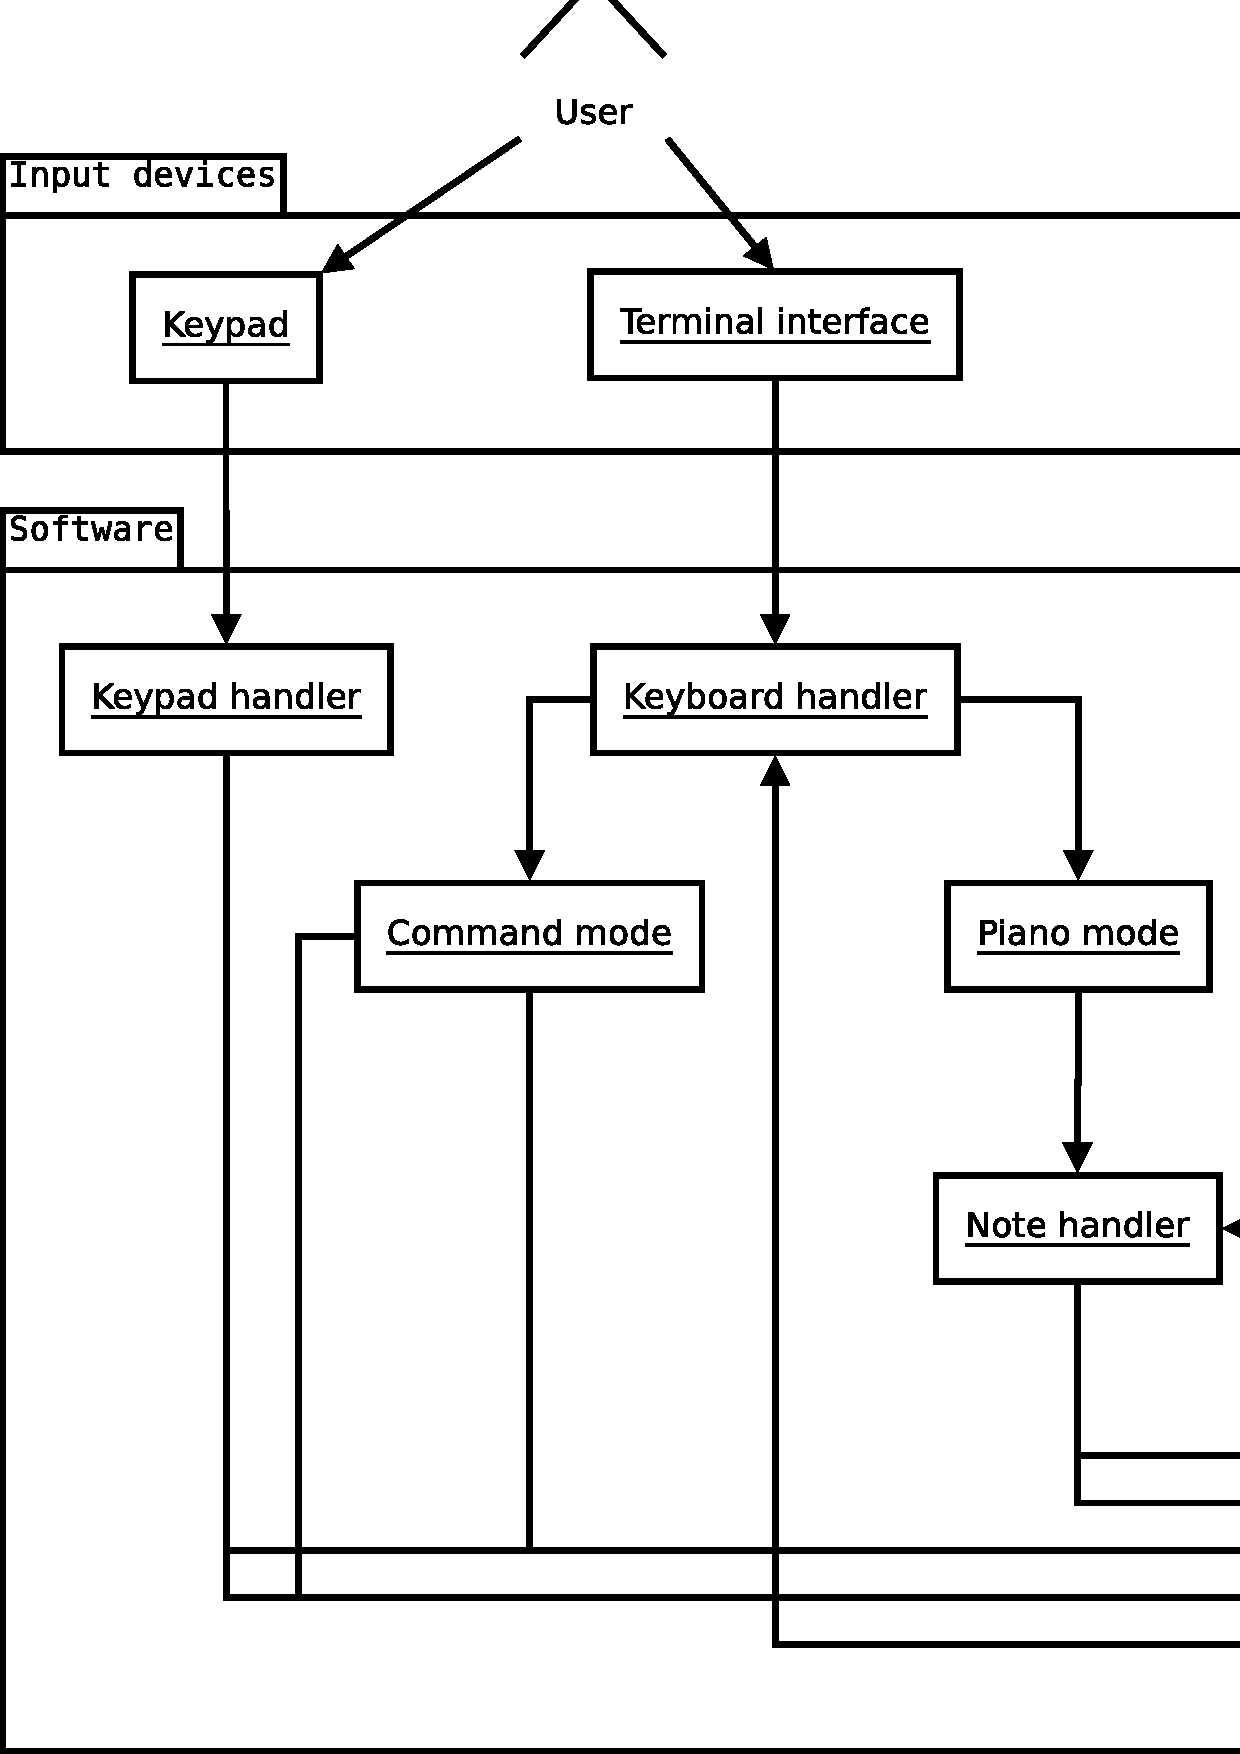
\includegraphics[totalheight=0.55\textheight,angle=90]{images/overview.png}
\caption{System overview}\label{fig:systemoverview}
\end{figure}

The diagram in Figure \ref{fig:systemoverview} shows the conceptual architecture of my system.  The 
basic idea is that various inputs are processed and in some way modify the state of the system, and 
this state in turn affects the operation of the continuously-running wave table playback.

The most important element of the system is the real-time conversion of network data to audio.  The 
network interface is a serial connection with a 19200bps baud rate.  Data arrives at a rate of one 
34-byte packet every 34ms.  The data format is sixteen pairs of bytes, each pair containing a MIDI 
note value and a volume level (both in the range 0--127), with each pair representing a channel 
between 0 and 15 (in order), and the packet is terminated with a null byte (00h) and a carriage 
return (0Dh).  The mapping of channel identifiers to instruments is shown in Table 
\ref{tab:channelids}.  For the ``Percussion'' channel, the volume level represents the particular 
percussion instrument to play rather than the volume at which to play it.

\begin{table}[htbp]
\centering
\begin{tabular}[bp]{c l}
ID & Instrument \\
\hline
0 & Bass Guitar \\
1 & Cello \\
2 & Church Organ \\
3 & Piano \\
4 & Saxophone \\
5 & Melody \\
6 & Violin \\
7 & Trombone \\
8 & Trumpet \\
9 & French Horn \\
10 & Synth \\
11 & Electric Guitar \\
12 & Acoustic Guitar \\
13 & Flute \\
14 & Piccolo \\
15 & Percussion
\end{tabular}
\caption{Network data channels}\label{tab:channelids}
\end{table}

\subsection{Network}

% FIXME: contradiction with actual design?
The network handler deals with collecting data from the incoming bytes on the serial interface 
connected to the network and running the packet handler when the end of a packet is detected.  The 
carriage return is interpreted as the end of the packet, and the incoming bytes are counted and 
checked to detect and ignore incomplete packets.

When the end of a complete packet is detected, the packet handler is run.  The volume is converted 
from a 7-bit to 8-bit value and sent to the volume output, and also converted to hexadecimal and 
displayed on the LCD.  The MIDI note is used as the index in a lookup table for the PRT reload value 
and wave table divisor (see \ref{wavetables}), and also in another lookup table for a 4-character 
representation of the note which is shown on the LCD.

\subsection{Wave tables}
\label{wavetables}
% TODO: double check the maths!

In my design, all frequencies of the instruments are synthesised from the same wave table sample, 
therefore a way is needed to perform this frequency conversion.  A sample has two important 
interdependant properties --- the sample rate and the frequency.  When changing either of these 
properties, the following property holds:

\[\frac{F_{target}}{F_{source}} = \frac{R_{target}}{R_{source}}\]

In other words, if a particular note is recorded at a particular sample rate, then the difference of 
the frequency when played is proportional to the sample rate it is played at.  In this case, we are 
aiming to play a particular frequency, so the required sample rate can be calculated with:

\[R_{target} = \frac{F_{target} \times R_{source}}{F_{source}}\]

Unfortunately, at higher playback frequencies the necessary sample rate will be impractically high, 
so an additional way of changing the frequency is needed.  If for example only every other sample 
from the wave table is played, without changing the sample rate, this will double the frequency of 
the note being played, since the entire sample is being played twice as fast.  More generally, if a 
divisor $D$ is introduced, then $F_{target} = F_{source} \times D$.

To combine the two methods, $F_{target}$ can be replaced with $F_{target} \times D$.  With a little 
re-arrangement, the following equation can be obtained:

\[R_{target} \times D = \frac{F_{target} \times R_{source}}{F_{source}}\]

See \ref{notelookuptables} for how this conversion is implemented to generate the MIDI note lookup 
tables.

% vim: fo=aw2tq tw=100 spell
\section{Design and Implementation}

\subsection{Keypad handler}

The keypad is a slightly awkward device for trying to get a single value --- it interrupts the whole 
time that the key is being pressed.  When implementing the keypad handler, this was the main problem 
I had to overcome.

My solution was to create a kind of lockout for that particular interrupt handler.  The result is a 
variable that acts as an ``already handled'' flag for keypad interrupts.  When a keypad interrupt 
happens, the flag is checked --- if it's non-zero, then the interrupt gets effectively ignored.  If 
it's zero, the interrupt handler executes as normal.  At the end of the interrupt handler, there are 
a few NOP instructions before setting the lockout variable back to zero and returning from the 
interrupt, but \emph{after} the interrupts are re-enabled.  The idea is that if the key is still 
pressed, it will interrupt during those NOPs, before the flag is cleared, and those interrupts will 
get ignored, but on the very last interrupt it will complete the handler.  This completely 
eliminates the possibility of accidental repeats.

For comparison, the alternative solution was to insert a delay after handling the keypress to allow 
time for the key to be released.  Unfortunately, that method was less than ideal, since if the delay 
was too long it would result in the system seeming unresponsive, and if too short then repeated 
interrupts would occur.  I felt it was better to maintain a direct responsiveness between action and 
reaction.

\subsection{Note lookup tables}
\label{notelookuptables}

Lookup tables are needed to contain the PRT value, divisor and note name (including octave) for 
every MIDI note.  The note names are in a separate lookup table to the other data as having an LCD 
information display was a lower priority than working sound playback and was implemented much later.

% TODO: expand on comparison of formats
The most efficient way to use a lookup value for a table is to multiply it by a power of two (left 
shifting), so blocks of data in the lookup table are also going to be $2^n$ bytes long.  However, 
the data for note playback is 3 bytes (a 16-bit PRT value plus an 8-bit divisor), so I was faced 
with the choice of having two lookup tables for the playback data or wasting $\frac{1}{4}$ of the 
space used by the table.  After writing the necessary assembler for reading from both possible 
formats and analysing their execution times, I found that the single table method resulted in faster 
code.  Combined with the fact I was not under pressure to conserve memory, I chose the single table 
method.

% TODO: expand on the result sorting
The Python script\footnote{"tools/pitchtable.py" in the submitted source code} I wrote to generate 
the lookup tables\footnote{"note\_lookup.s"} is based on the concept outlined in \ref{wavetables} 
for creating new frequencies from a single sample by modifying the sample rate and divisor.  PRT and 
divisor values are calculated for the frequency information in the pitch 
table\footnote{"tools/pitchtable.csv" - octave, MIDI note number, note name, frequency}.

The first step is calculating the PRT value for every divisor, $D$ from 1 to 255, first by 
calculating the sample rate using

\[R_{target} = \frac{F_{target} \times R_{source}}{F_{source} \times D}\]

(rearranged from a similar equation in \ref{wavetables}) and then converting this to a PRT value 
using

\[PRT = round\left(\frac{F_{CPU}}{D_{PRT}\times{}R_{target}}\right)\]

where $F_{CPU}$ is the CPU frequency (6,144,000) and $D_{PRT}$ is the PRT divisor (20).  Because the 
result has been rounded to the nearest integer, the effective frequency will be different to the 
desired frequency.  The effective frequency is calculated by using the $PRT$ and $R_{target}$ 
calculations in reverse:

\[F_{effective} = \frac{F_{source}\times{}D\times{}\frac{F_{CPU}}{D_{PRT}\times{}PRT}}{R_{source}}\]

The error, E is calculated with the following, giving a value in the range 0--1:

\[E = \frac{\left|F_{effective} - F_{target}\right|}{F_{target}}\]

% TODO: to joke or not to joke?
For each note, the results for all the divisors are collected together, discarding those where the 
sample rate is higher than 8kHz (a sensible limit given the CPU speed), and sorted in reverse order 
by $R^{1-E}$.  The idea is that the basic ordering aims for a high sample rate, but any kind of 
significant error greatly diminishes the value of the result.  The first result is taken from the 
sorted list, giving the PRT and divisor values the algorithm decides best represent the frequency.  
While almost seeming like mathematical voodoo, the worst error rate for any note in the resulting 
table is $1.13\%$, with an average sample rate of just under 7kHz.  Other sorting methods I tried 
had varied results, generally creating high sample rates with high error margins, or low error 
margins with bad sample rates.

The format of the resulting lookup table is:
\begin{center}
\begin{tabular}{c | c | c | c | c}
Byte & 0 & 1 & 2 & 3 \\
\hline
Usage & PRT low & PRT high & Divisor & 00h \\
\end{tabular}
\end{center}

The script also produces a second table which contains a 4-character representation of the note 
created from the octave number and note name.

% vim: fo=aw2tq tw=100 spell
\chapter{Testing and Evaluation}
\label{sec:testing}

This section is a commentary on the testing procedures used throughout the project.  My general 
approach was bottom-up iterative development and testing---starting with the most basic components 
that stand on their own, testing them thoroughly, and building the next layer of complexity on top 
of them.  Every component that is tested well and known to be working provides a good stable 
platform for testing other components against.

\section{Output Hardware}
\label{sec:testing:hardware}

Using the principle of testing components with already working components, it made sense that the 
first part that needed to be tested was the audio hardware.

After assembling the audio output hardware as designed (and illustrated in 
Appendix~\ref{appendix:circuit-diagram}), but before connecting the data lines to the parallel I/O 
ports, the behaviour was tested manually by setting input values with 8-bit DIP switches, and 
measuring voltages with an oscilloscope.

First, both inputs were set to the maximum values, and the voltage measured from the output of the 
second op-amp (IC4, pin 6).  This is the maximum voltage.  Starting from the MSB, each bit of the 
input to the volume DAC was switched from ``on'' to ``off'', and the voltage observed at each point.  
The voltage was halved for every bit turned off, as expected.  This showed that the first DAC was 
operating correctly, and that the ``pre-scaling'' effect also worked correctly.

The experiment was repeated, but this time changing only the value of the waveform DAC.  The same 
results were observed, as expected.  This means this DAC was also working correctly.

Next, an 8-bit binary counter was assembled and run as the input to each DAC in turn to test the 
response to changing inputs.  The observed waveform on the oscilloscope revealed overshoot in the 
output when the value changed.  Fixing this issue is described in 
Section~\ref{sec:design:hardware:feedback}.  Other than this, the device performed as expected.

The oscilloscope probe was then moved to the output of the audio amplifier.  Since a binary counter 
provides a sawtooth wave, the previous test was already providing the maximum jump between values.  
We found that if we turned the potentiometer to its maximum value, the top of the wave would be 
clipped, however through most of the range the waveform was correct.


\section{Output Interface}

Testing the software interface to the output device was as simple as writing a simple loop program 
to cycle through a mock waveform, at three different volumes.  I did this for a simple 8-point 
``sine'' wave, which displayed as expected (not anything like a sine wave because of the short 
transition time) --- this also gave me an idea of the maximum rate at which the output device could 
be driven, since there was no delay inserted in the loop.

\section{PRT-Based Playback}

A program was created which used a PRT interrupt to drive the playback.  The interrupt handler 
alternated between 00h and FFh, giving a square wave.  The tests mainly involved obtaining specific 
frequencies by setting the PRT reload register value.

\section{Wavetable Playback}

When I implemented PRT-based wavetable playback, the startup routine of the software involved 
setting the device playing a particular note.  A single 256-sample 2-wave sine wavetable was created 
for testing the software (instrument samples were left till later in the project once everything 
else was working).  The oscilloscope probe was attached to the amplifier output so I could see the 
output waveform and check that it matched what should be output.  Figure~\ref{fig:oscilloscope} 
shows the oscilloscope when playing one of the final instrument samples.

\begin{figure}[htb]
\centering
\includegraphics[width=0.7\textwidth]{images/oscilloscope}
\caption{Oscilloscope Trace of Amplifier Output}\label{fig:oscilloscope}
\end{figure}

\section{Terminal Interface}

Testing the terminal interface was a simple matter of echoing back everything sent to the device.  
After this, sending stuff to the terminal could be used as a diagnostic for other parts of the 
software.

\section{Network Interface}

In the first instance, testing the network interface was set up correctly was a matter of echoing 
everything received to the terminal --- this at least verified that something was arriving.

Testing that the correct data was being received was more subjective.  This involved listening to 
the audio output to make sure it sounded right.  The most common error I had which could be heard 
was using the volume data as the note --- this has a very distinctive sound because of the volume 
decay in the network data.

\section{LCD Text Display}

Testing the LCD text display functions I wrote just involved writing some characters to different 
positions on the screen.

\section{Keypad Interface}

Testing the keypad interface was done by making the keypad handler output the value of the key 
pressed to the terminal.

% vim: fo=aw2tq tw=100 spell
\chapter{Technical Specification}

\section{Functionality}
\label{sec:spec:functionality}

\section{Cost}
\label{sec:spec:cost}

\begin{center}
\begin{tabular}{c | c | r | r}
Part & Quantity & Per-unit & Total \\
\hline\hline
DAC0832LCN              & 2     & \pounds1.66 & \pounds3.32 \\
LM356N                  & 2     & \pounds0.40 & \pounds0.80 \\
LF386N-1                & 1     & \pounds0.26 & \pounds0.26 \\
$8\Omega$ speaker       & 1     & \pounds2.62 & \pounds2.62 \\
$10K\Omega$ potentiometer & 1     & \pounds0.72 & \pounds9.72 \\
Metal film resistor ($\pm1\%$)    & 3     & \pounds0.06 & \pounds0.18 \\
Electrolytic capacitor  & 5     & \pounds0.08 & \pounds0.40 \\
Ceramic capacitor       & 5     & \pounds0.07 & \pounds0.35 \\
PCB manufacture (40mm $\times$ 40mm) & 1     & \pounds2.90 & \pounds2.90 \\
\end{tabular}
\end{center}

Component prices quoted from Farnell UK.  PCB manufacture quoted from PCBTrain quote 
calculator\footnote{\url{http://www.pcbtrain.co.uk/onestepquote.php}}.  Prices correct as of 
07/04/2008.  Based on a batch of 100 units.

% vim: fo=aw2tq tw=100 spell
\section{Further Work}

% Merging the 2 MIDI lookup tables into one


\appendix

\section{Circuit diagram}
\label{appendix:circuit}
\begin{center}
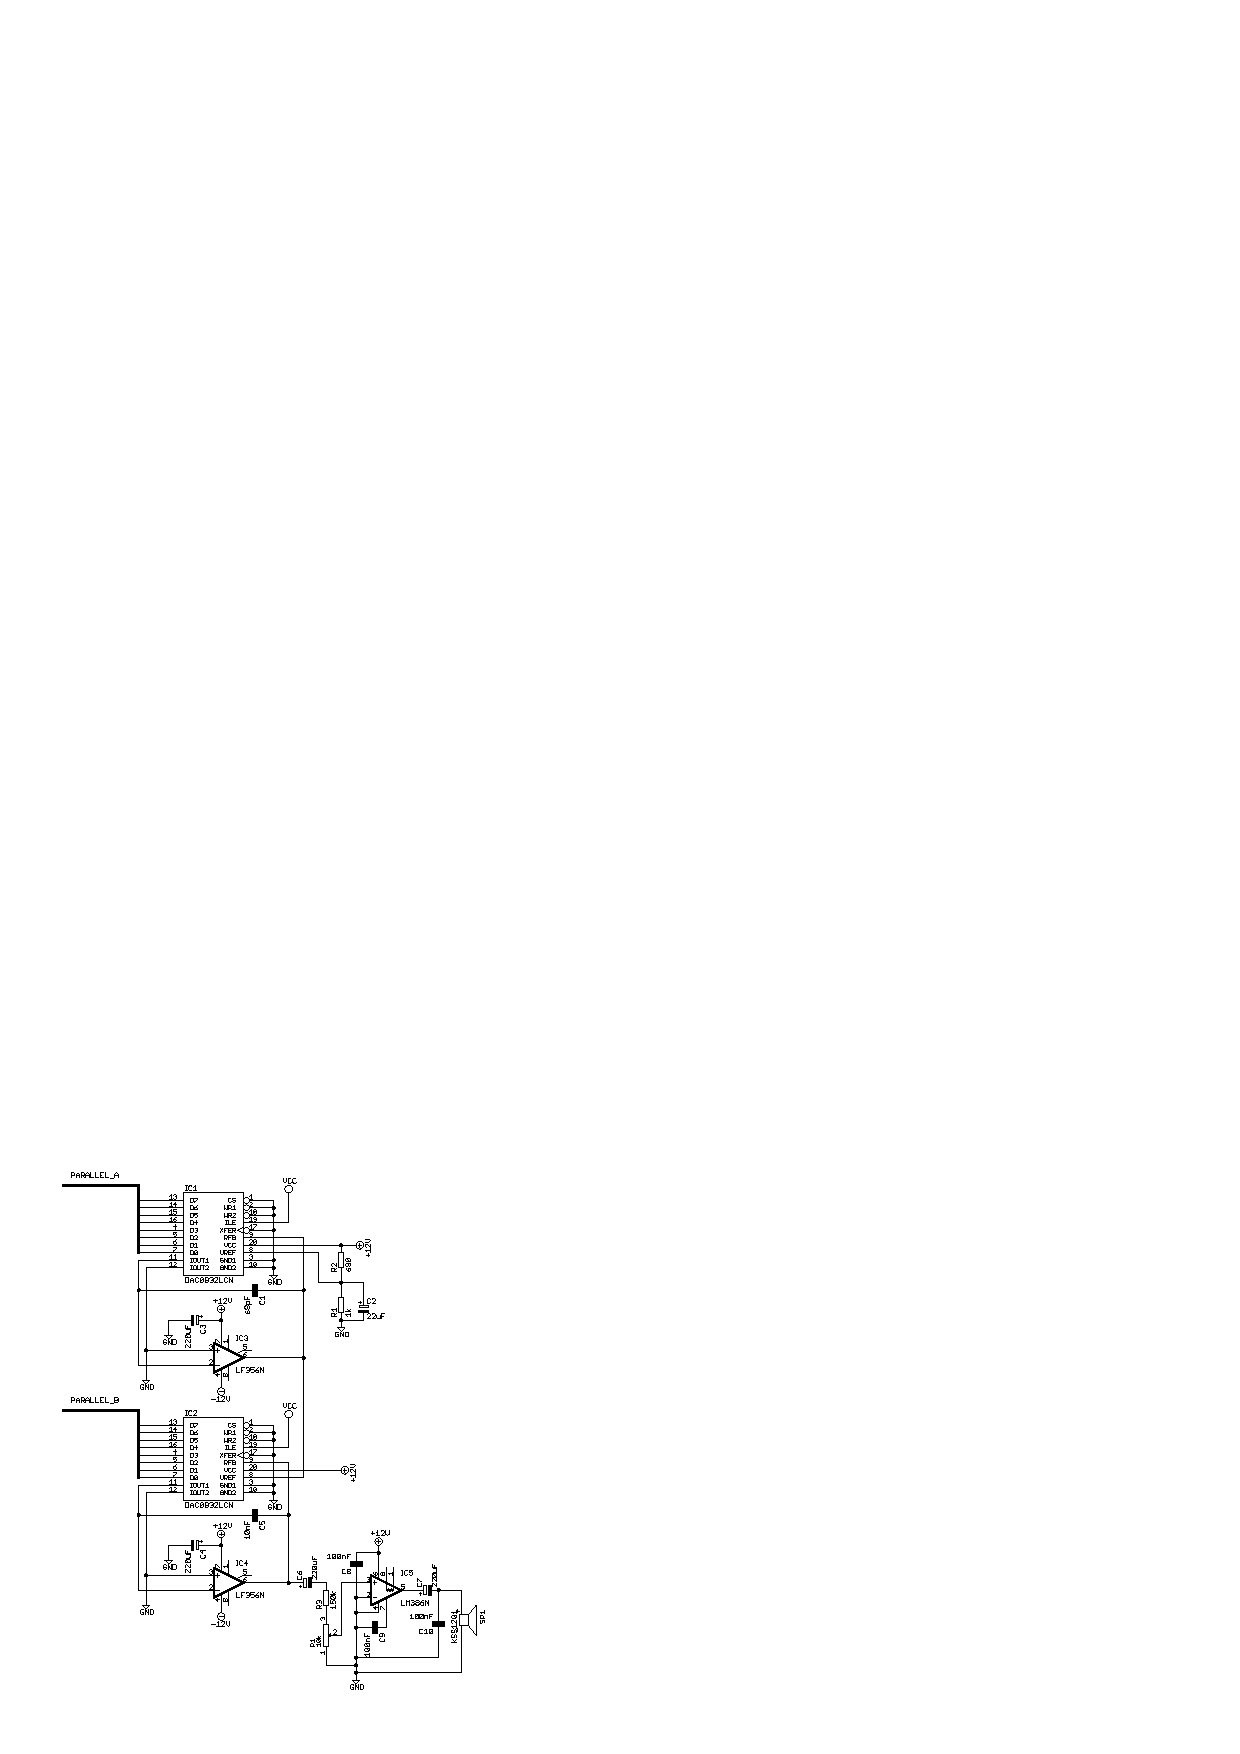
\includegraphics[totalheight=0.95\textheight]{images/output-schematic.png}
\end{center}


\pagebreak
\begin{thebibliography}{99}
% \bibitem{ref}Author:
% \emph{Title},
% \url{http://} (year)
\end{thebibliography}

\end{document}
